%\documentclass{beamer}
%\usetheme{Pittsburgh} 
\documentclass{scrartcl}

\usepackage[utf8]{inputenc}
\usepackage{default}
\usepackage[procnames]{listings}
\usepackage{graphicx}
%\usepackage[toc,page]{appendix}
\usepackage{caption}
\usepackage{hyperref}
\usepackage{color}
\usepackage{float}
\usepackage[T1]{fontenc}

%Python
\definecolor{keywords}{RGB}{255,0,90}
\definecolor{comments}{RGB}{0,0,113}
\definecolor{red}{RGB}{160,0,0}
\definecolor{green}{RGB}{0,150,0}
\lstset{language=Python,
basicstyle=\ttfamily\scriptsize,
keywordstyle=\color{keywords},
commentstyle=\color{comments},
stringstyle=\color{red},
identifierstyle=\color{green},
procnamekeys={def,class},
breaklines=true,
columns=fullflexible,
%Numbering and Tabs
%numbers=left,
%tabsize=4,
%showspaces=false,
%showstringspaces=false
}


%Bibliogrpahy?
%\usepackage{bibentry}
%\nobibliography*
%\bibentry{ }


\begin{document}

\title{Evolutionary Computation Theory and Application}
\subtitle{Report}
\author{
  Quignon, Christophe \\
  \href{https://github.com/ChrisQuignon/ECTA}{github.com/ChrisQuignon/ECTA}
  %Familyname, Name
} 
\date{\today}


\maketitle


\setcounter{tocdepth}{2}
\setcounter{secnumdepth}{2}
\tableofcontents{}


\section{Optimization}
%Theoretic description
The first exercise was about the performance of different optimization algorithms on landscapes with raising complexities. The algorithms where simple and had little tuning parameters. They function similar to genetic algorithms by iteratively improving their performance. But they do not run in populations, there is no random mutation and no crossover. 

\subsection{Problem}
\subsubsection{Square error}
The square error function has only one optimum and is among the most simple optimization problems. Only a a very bad parameter choice could lead to not finding an optimum.

\subsubsection{Trimodal fitness function}
The trimodal fitness function has two local optimum and a global optimum in between them. It is simple but can be used to illustrate the problem of overcoming local optima.

\subsubsection{3D plateau fitness function}
The 3D plateau fitness function is more complex then the functions before. It stretched 3 dimensions and not only 2 and has plateaus which are also tricky to overcome. This complexity already ruled out the newton method, because the derivative in 3D is tricky to implement.
%characteristics of the problem

\subsection{Algorithms}
%How do we solve it
\subsection{Hillclimber}
The Hillclimber method is an effective an easy way to find a local optimum by iterative evaluation of all neighbouring points and choosing the best of those. It can be optimised by evaluating more neighbours but can not overcome local optima beyond the reach of the neighbours.
\subsubsection{Basic Steepest Descent}
The steepest descent is a variant of the Hillclimber. It does not evaluate the neighbours fitness itself but the gradient towards the neighbours. By following the gradient it converges faster than the Hillclimber.
\subsubsection{Steepest Descent with momentum}
The steepest descent method can be augmented by introducing a moment to the size of steps. That way it can overcome local optima. The momentum itself is defined by the last step width and scaled by the inertia.
\subsubsection{Newton’s Method}
In Newtons method the step width is derived by the first and second gradient of the neighbourhood of the function. Therefore it is very effective but requires exact knowledge of the function and its derivatives, which are not known for more complex problems.

\subsection{Parameters}
%What could be changed
\subsubsection{Precision}
The precision is used to determine when the algorithm no longer improves. for all runs it is set to 0.0001
\subsubsection{Starting Positions}
The starting positions highly impact the performance of a single run. In this scenario they are evenly spaced in the range of the landscape. In other scenarios it might be more practical to choose them at random.
\subsubsection{Learning Rates}
The learning rate is the factor by which the step width is increased or decreased per iteration. The learning rates typically are quite small. For the analysis they where:\\
 0.0,  0.004,  0.00711312,  0.01264911, 0.02249365, 0.04,  0.07113118,  0.12649111,  0.22493653,  0.4.  (logspace(0, 2, 9)/250)
 The logarithmic distribution allows for a granular analysis in lower ranges and a good prediction for higher values.
\subsubsection{Momentum}
The momentum is defined by the inertia used to calculate it. A higher inertia means a lower adaptation rate. The values chosen where the same as for the learning rates. An inertia of zero was interpreted as no momentum.

\subsection{Analysis}
%what happened and why
All of the algorithms performed very well on all landscapes. They found an optimal value typically within 50 iterations. The Newton method performed best and found the optimum of the squared error with only one step. This was due to the nature of the function and its derivatives. But newton method also worked very good for the trimodal landscape.\\
The Hillclimber and the method of Steepest Descent almost all of the time found a local optimum. Only very low learning rates (or momentum) lead to a suboptimal termination after 50 iterations. On the other hand, very high learning rates or momentum (> 0.3) often led to a step width that did not reflect the surface and thus results in an unpredictable behaviour.\\
Especially in the 3D landscape this often led to points outside of the defined ranges. (See Figure \ref{fig:plateau})

%PLATEAU
\begin{figure}[H]
\centering
\begin{minipage}{.5\textwidth}
  \centering
  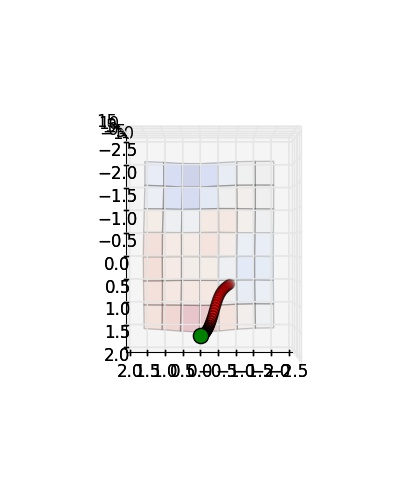
\includegraphics[width=.8\linewidth]{img/ex1/runs/SD-Plateau3D_0_0,07.jpg}
  %was SD-Plateau3D_-0.81  0.59_0.0_0.07
  %\caption{}
  %\label{fig:}
\end{minipage}%
\begin{minipage}{.5\textwidth}
  \centering
  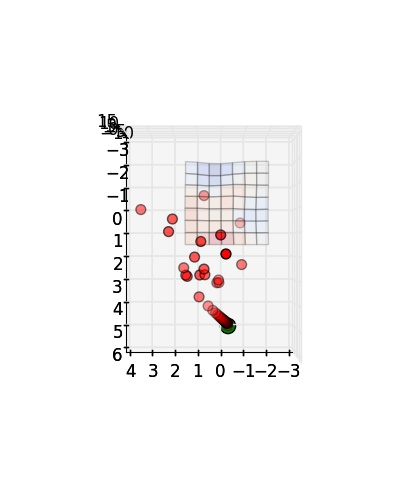
\includegraphics[width=.8\linewidth]{img/ex1/runs/SD-Plateau3D_0,22_0,02.jpg}
  %\caption{}
  %\label{fig:} 
\end{minipage}
\caption{Two highly different runs of the steepest descent algorithm in the Plateau3D landscape. Learning rates of 0.0 (left) and 0.22 (right) and inertia 0.07 (left) and 0.02 (right).}
\label{fig:plateau}
\end{figure}

\subsubsection{Fitness}
Since the algorithms are deterministic for a given set of parameters, it is not necessary to build the mean over a couple of runs. Instead the performance was analysed with respect to to the parameters.\\

\paragraph{Starting position}
The starting position has a huge impact on the performance because it define whether the next optimum is a local or a global one, and how far the algorithm needs to travel. For a 2D landscape the minimum fitness assembles the fitness landscape, while the maximum fitness should point out the optima. As seen in Figure\ref{fig:2dminmax} the optima of the squared error was found independent of the starting position where for the trimodal landscape the Hillclimber (dashed) sometimes could not find a optimum. 
%MEANMAX
\begin{figure}[H]
\centering
\begin{minipage}{.5\textwidth}
  \centering
  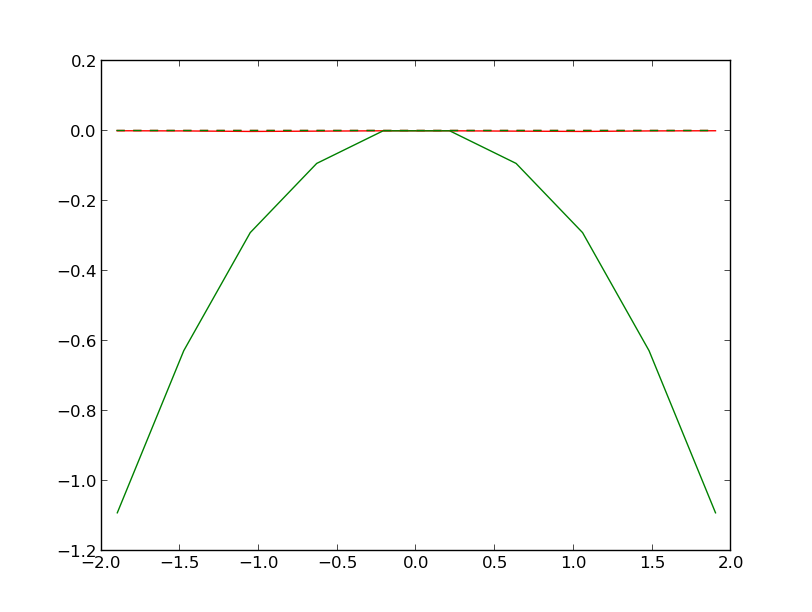
\includegraphics[width=.8\linewidth]{img/ex1/analysis_squared_newton_hill.png}
  %\caption{}
  %\label{fig:}
\end{minipage}%
\begin{minipage}{.5\textwidth}
  \centering
  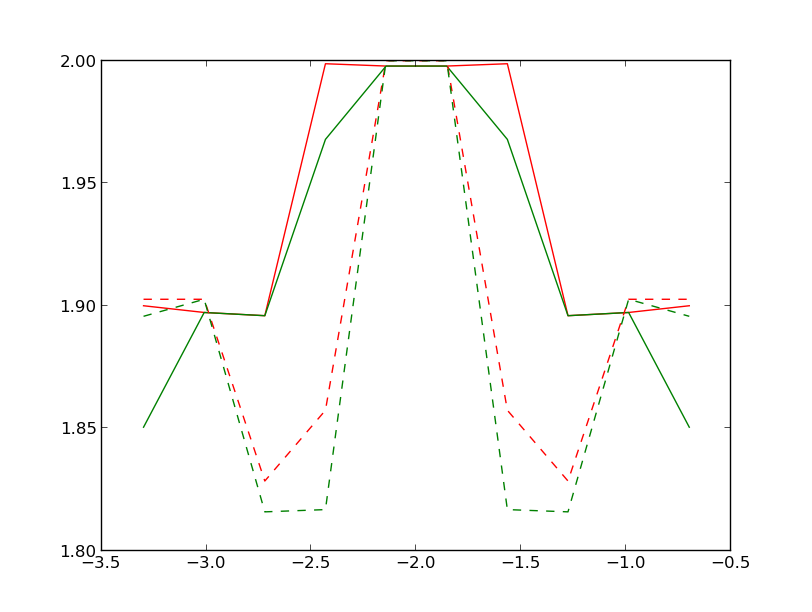
\includegraphics[width=.8\linewidth]{img/ex1/analysis_trimodal_newton_hill.png}
  %\caption{}
  %\label{fig:} 
\end{minipage}
\caption{Fitness analysis of the mean (green) and maximal(red) values of the newton method (solid) and the Hillclimber (dashed).}
\label{fig:2dminmax}
\end{figure}
%Description

In the 3D landscape, the fitness was analysed by a heat map that maps the final fitness to the starting position. All areas of the same colour converge to the same fitness. As seen in Figure\ref{fig:heatmap} the Hillclimber often gets stuck at the plateau (blue). With the given parameters, the Hillclimber performed more reliable because it did not overshoot. With the right parameters, the steepest descent did perform better.
 
%HEATMAPS
\begin{figure}[H]
\centering
\begin{minipage}{.5\textwidth}
  \centering
  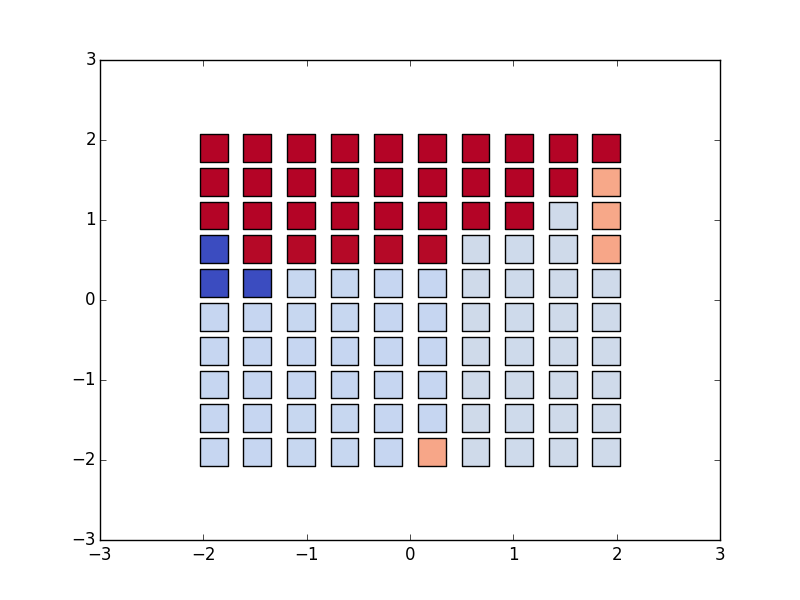
\includegraphics[width=.8\linewidth]{img/ex1/Heatmap_HC.png}
  %\caption{}
  %\label{fig:}
\end{minipage}%
\begin{minipage}{.5\textwidth}
  \centering
  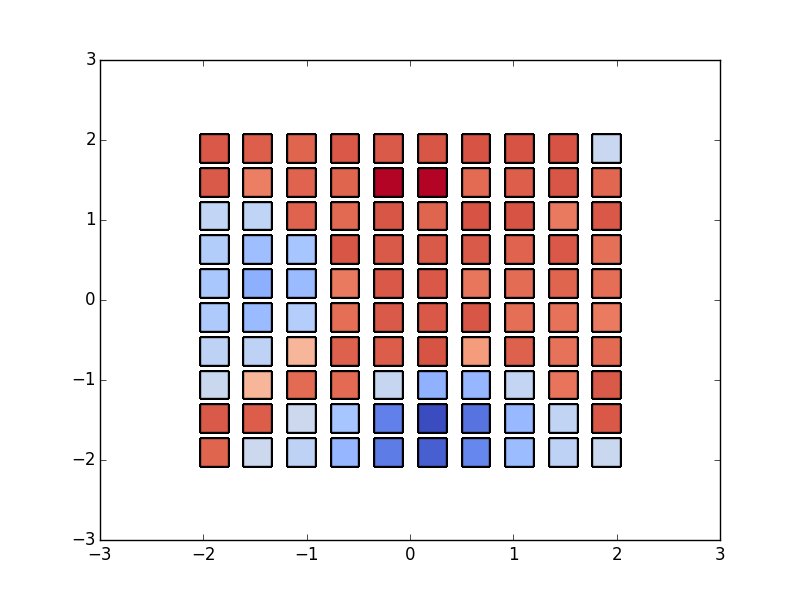
\includegraphics[width=.8\linewidth]{img/ex1/Heatmap_SS.png}
  %\caption{}
  %\label{fig:} 
\end{minipage}
\caption{Heatmap of the fitness values of the Hillclimber (left) and Steepest Descent(right) method in a 3D Landscape.}
\label{fig:heatmap}
\end{figure}

\paragraph{Step width}
The step width is determined by the learning rate and the inertia. Both are crucial to overcome local minima. In Figure \ref{fig:inertialearning} Those parameters are grouped and all final fitness are shown as individual dots. This allows to see how often one parameter reaches an optimal fitness.
As the fitness for the squared error is global by nature and the overshoots in the 3D case, only the trimodal landscape is shown.\\
From the point density one can see that the learning rate(left) is a more reliable way to point towards an optimum while the inertia(right) overcomes the local minima at 1.0 better.

%INERTIA LEARNING
\begin{figure}[H]
\centering
\begin{minipage}{.5\textwidth}
  \centering
  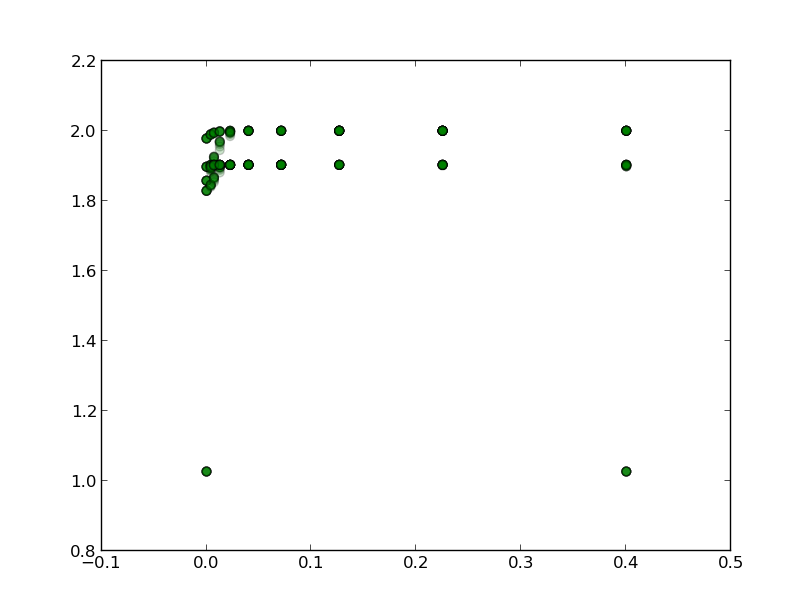
\includegraphics[width=.8\linewidth]{img/ex1/learning_trimodal_ss.png}
  %\caption{}
  %\label{fig:}
\end{minipage}%
\begin{minipage}{.5\textwidth}
  \centering
  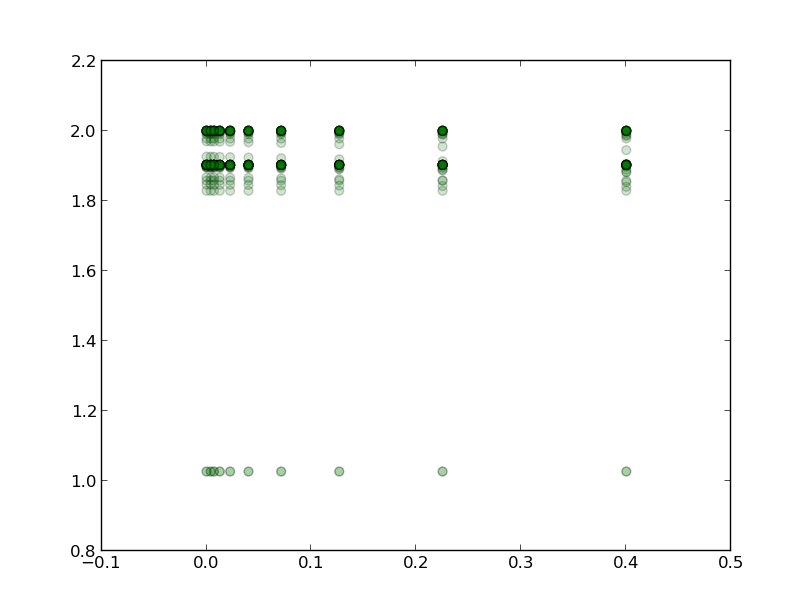
\includegraphics[width=.8\linewidth]{img/ex1/inertia_trimodal_ss.png}
  %\caption{}
  %\label{fig:} 
\end{minipage}
\caption{Comparison of the fitness values with respect to the learning rate (left) and inertia(right) with the steepest descent method on the trimodal landscape.}
\label{fig:inertialearning}
\end{figure}

\subsubsection{Best result}
To discuss the fitness optimality on these landscapes does not give any insight because almost all runs where successful. However the steps to reach the goals varied, as as shown in Figure \ref{fig:stepssquared}. The Hillclimber took the most steps, while the steepest descents found the optimal quickly. The fastest however has the newtons method.

%RUNS
\begin{figure}[H]
\centering
\begin{minipage}{.5\textwidth}
  \centering
  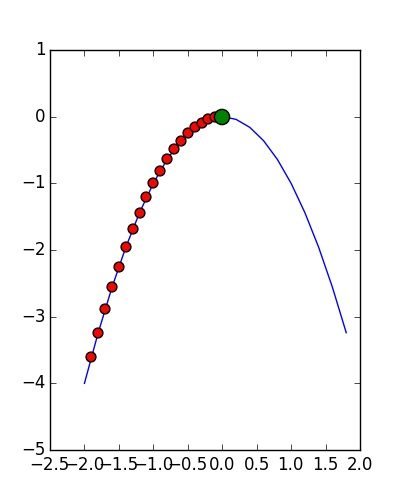
\includegraphics[width=.8\linewidth]{img/ex1/runs/HC-SquaredError2D_-1,9.jpg}
  %\caption{}
  %\label{fig:}
\end{minipage}%
\begin{minipage}{.5\textwidth}
  \centering
  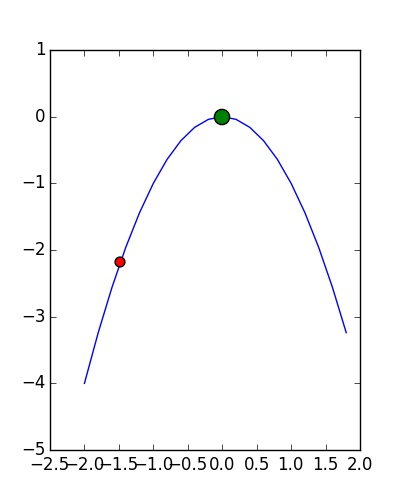
\includegraphics[width=.8\linewidth]{img/ex1/runs/NM-SquaredError2D_-1,48.jpg}
  %\caption{}
  %\label{fig:} 
\end{minipage}
\caption{Incrementing steps of optimization of the Hillclimber (left) and the Newton Method (right) on the squared error landscape.}
\label{fig:stepssquared}
\end{figure}


\subsection{Conclusion}
The varying complexity of the fitness landscape and the degree of information about the landscape used in the algorithms had to match to show a good performance. Thus, the Hillclimber as a mostly uninformed method did a good job on all landscapes but can not overcome local optima. The performance was increased by adapting the step width and direction with a learning rate or the information about the steepest descent. Those however require tuning or additional information. The most complex and effective algorithm, Newtons method performed best.\\
So if we have no additional information about the landscape to optimize, parameter tuning is required. If we have additional information, this can greatly improve the performance. This however is not a likely scenario.



\section{Genetic Algorithms}
%Theoretic description
In the second exercise, the same problems where approached with a genetic algorithm. A given population run some iterations through the basic algorithm to find the optimum of the function. The single steps of the algorithm, namely:\\

\begin{itemize}
\item evaluation
\item selection
\item crossover
\item mutation
\end{itemize}

The single steps where varied to explore the possibilities of genetic algorithms and to find an optimal parameter set. The variations are given in the Algorithm section.



\subsection{Problem}
%characteristics of the problem
The problems where given by the same fitness functions as in the exercise before.

\subsection{Algorithms}
%How do we solve it
The most significant difference in the algorithm is the type of crossover. The recombination of two individuals can be based on two representations of their genotype:
\begin{itemize}
\item string based
\item real valued based
\end{itemize}

Depending on the type we can either use arithmetic functions to create an offspring or manipulations based on the string or bit representation.

\subsection{Parameters}
%What could be changed
\subsubsection{Population size}
The population size defines the number of individuals that are evaluated every iteration. The higher it is, the more variety in can hold. This variety however depends on the mutation and crossover and is not due to the population size. \\
The values tested where 10, 50 and 100. 

\subsubsection{Selection}
The selection determines which individuals where carried over into the next iteration and which where replaced. In the evaluation method, the individuals where ordered by their fitness value. The selection of the best individuals where given as a percentage value of the population size.\\
The values tested where 10\%, 50\% and  100\%

\subsubsection{Crossover}
From the pool of selected individuals, a new population is generated. Two of the selected individuals are picked at random (possibly choosing the same individual) and forming an offspring by one of the three crossover types per representation:

\begin{enumerate}
\item Real valued representation
	\begin{itemize}
	\item Mean\\
	The arithmetic mean of the point values where passed to the offspring. This restricts the value of the offsprings with every step, because the mean value can not leave the range of the given values.
	\item Fitness mean\\
	In this variant, the mean is weighted by the fitness values of the offspring. This pushed the mean towards the parent with the higher fitness. The same problem as with the regular mean applies. 
	\item Randomly weighted mean\\
	Here the weighting happens at random, allowing for a more diverse distribution of the offspring within the bounds of its parents. The same problem as with the regular mean applies. 
	\end{itemize}
\item String representation
	\item N-point crossover.\\
	The strings where of the float values where crossed over at one, two or three points. The first crossover point was the "." in the float, switching the modulo and the div values of the strings. Subsequently the modulo sub strings where switched at the 2nd and also at the 3rd position.
\end{enumerate}

An example of the n-point crossover would be:

\begin{itemize}
\item Parent one: -1.2345
\item Parent two: 6.789
\begin{itemize}
	\item One point crossover: -1.789
	\item Two point crossover: -1.7345
	\item Three point crossover: -1.739
	\end{itemize}
\end{itemize}
 
This can lead to offspring outside of the ranges of the parents possibly resulting in invalid ranges. However the effect of the crossover is smaller with bigger crossover numbers since the position significance decreases.\\
To no loose the currently best solution, the best individual is carried over into the new population without crossover and mutation. This method is called elitism.

\subsubsection{Mutation}
In every run, all individuals have a small chance to mutate. This will spread the points evaluated into possibly new regions but can also destroy good solutions. To counteract the destructive force of mutation, the mutation probability of the best individual was set to zero.
This probability was given in percentage.\\
The values tested where: 1\%, 10\ and 30\%]


\subsection{Analysis}
%what happened and why
%TODO
\subsubsection{Parameter variations}

\subsubsection{Fitness}

\subsubsection{Best result}

\subsection{Conclusion}



\section{Travelling Salesman}
%Theoretic description
In contrast to the first two exercises, the third one was concerned with simple functions and thus less artificial. To sole the problem, again a genetic algorithm was used. The problem however required to write an own fitness function and different selections, mutations and crossovers.\\
Focus in this exercise where the Building Block Hypothesis and the Schemata Theory both of which are discussed in the Analysis.

\subsection{Problem}
%characteristics of the problem

The travelling salesman problem is a famous problem in computer science to find the shortest circular path through a given set of locations. It is a NP-hard problem. The points given where the 100 biggest cities of Germany. It is noteworthy that the Ruhrgebiet in Germany is a small area in the west where a lot of large cities concentrate in a small area. In this area, a lot of paths are very close to each other and thus optimizing there does not increase the overall fitness. On the other hand, the probability to connect into the Ruhrgebiet is relatively high and will often lead to longer paths.

\subsection{Algorithms}
%How do we solve it
AS in exercise 2, a genetic algorithm was used. The range of variations in parameters however where reduced. The mechanisms for selection and mutation as well as elitism was used as before.

\subsubsection{Representation}
Two major ways to represent the path through all cities and back to the starting city where suggested:
\begin{itemize}
\item Priority list\\
Here the cities in random order get a float between zero and one assigned. The order of the float values are the order of cities on the path. This numeric representation allows for real value based mutation (as + 0.1) and crossovers independent of the position on the path but on the position in the unordered list.
\item Permutations\\
In the permutation representation, the cities are ordered by their position in a list. This allows for list based crossovers and mutations.
\end{itemize}

It is possible to represent all mutations in both representations and from a programming standpoint the representation must not have any influence on the mutation or any other part of the program.\\
Thus I choose to base my choice of representation not on the problem but on the programming language. Since Python is strong with lists and list manipulations, I kept the cities data unchanged and global, but represented the path as a list of indexes of the global city list. This the genome is a list of values between 0 and 99.

\subsubsection{Mutation}
In mutation, we flip the position of two randomly chosen cities on the path.

\subsubsection{Crossover}
For mutation, single point crossover was used. For two randomly chosen individuals a random index was chosen. Up to that index, the genome of parent one was used and the rest of indexes where filled in the order of parent two. In terms of path this means that we follow the path of parent one up to certain point and then continue the same way as parent two does.

\subsection{Parameters}
%What could be changed
In the analysis, three different variations of the parameters where chosen. Every parameter set was run 30 times and the min, mean and max fitness was recorded. Those then where plotted in groups by the values of the parameter. Green marks refer to a minimal value, red to a maximal value and blue to a mean.


\subsubsection{Population size}
The tested parameters for the population size where 10, 100 and 200.
In Figure \ref{fig:tsppop} it can be seen that the population size significantly impacts the min and mean values, while the max values stay high. The gaps inside the population sets indicate that the population size is not the main parameter to influence the fitness. The two gaps forming three groups per population parameter are likely to be one other parameter set of the values. The mean values are visibly better than the max values.

%TSP POP
\begin{figure}
 \center
 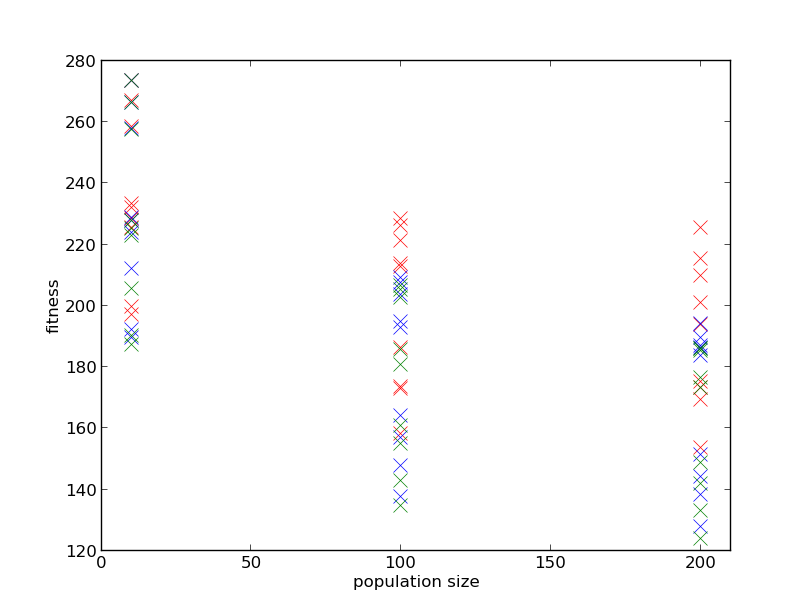
\includegraphics[width=.5\linewidth]{img/ex3/tsp_fitness_population.png} 
 \caption{All fitness values (min=green, mean = blue, max = red))ordered by population.}
 \label{fig:tsppop}
\end{figure}

\subsubsection{Selection rate} 
The selection rate as seen in Figure \ref{fig:tspselect} show two major significances. At first, a lower selection pressure contains more better fitness, second is that this correlation is not linear, since the highest selection rate is denser than the lower.\\
All three selection rates have one outlier to a very bad mean value. And only a little difference between the max and the min values.

%TSP Selection
\begin{figure}
 \center
 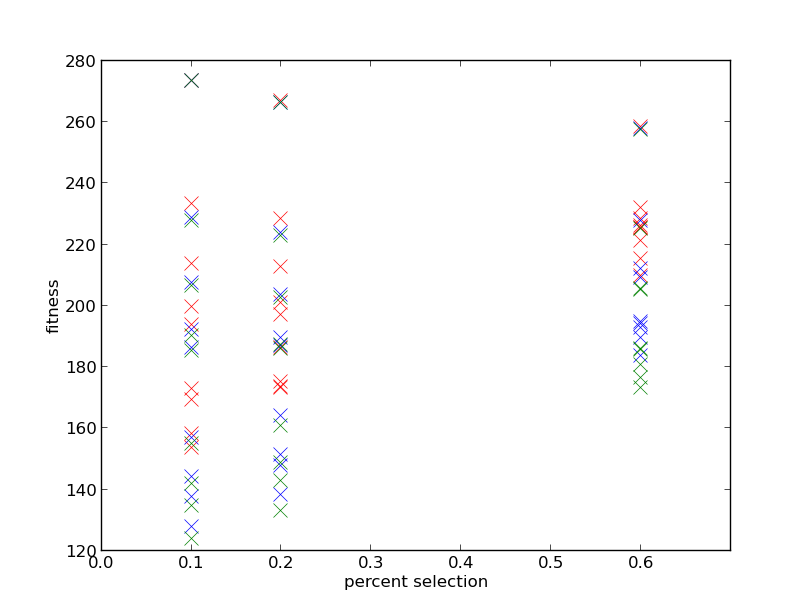
\includegraphics[width=.5\linewidth]{img/ex3/tsp_fitness_selection.png}
 \caption{All fitness values (min=green, mean = blue, max = red))ordered by selection pressure.}
 \label{fig:tspselect}
\end{figure}


\subsubsection{Mutation}
%TSP mutations
Figure \ref{fig:tspmutation} show the fitness values group by the mutation parameter. We again see big gaps inside the single parameters and a trend to a more widespread but in total better fitness when increasing the fitness. For higher mutations, the min value also has a greater distance to the max value.

\begin{figure}
 \center
 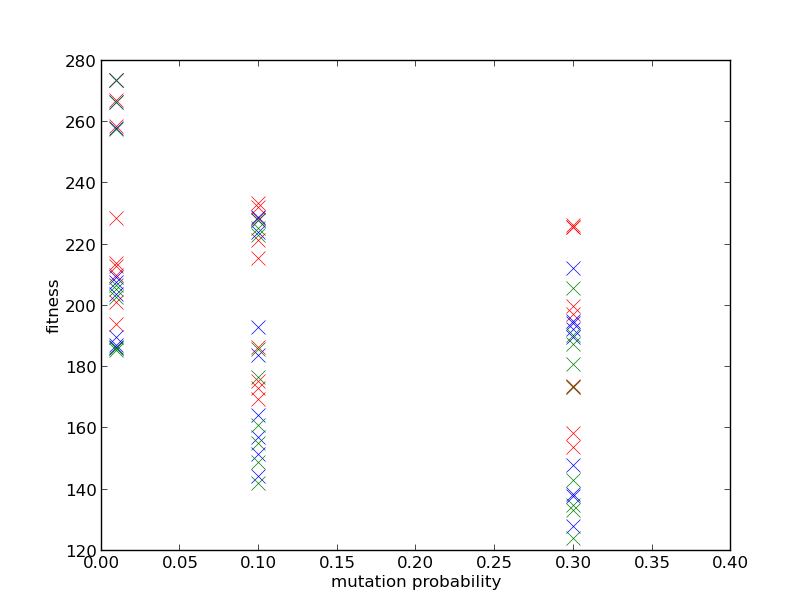
\includegraphics[width=.5\linewidth]{img/ex3/tsp_fitness_mutation.png}
 \caption{All fitness values (min=green, mean = blue, max = red))ordered by selection mutation.}
 \label{fig:tspmutate}
\end{figure}

\subsection{Analysis}
%what happened and why
The results of the analysis per parameters revealed a nontrivial connection between them and the algorithm itself. With the help of the Building Block Hypothesis and the Schema Theory it however was possible to project the results of the analysis onto other parameter values.\\
A helpful visualisation of the effects of mutation and crossover is the tracking of the best fitness. Over time it will converge to an optimum, but sometimes it will be drawn back, if the optimal solution is mutated. If the solution is a strong one, it will recover from the population. (See \href{https://www.youtube.com/watch?v=9m4KxnW7dLc}{youtube.com/watch?v=9m4KxnW7dLc}

\subsubsection{Building Block Hypothesis}
The Building Block Hypothesis says that in population of individuals the genotype can be grouped into building blocks that are wide spread because they are an efficient part of the solution. The spread of those building blocks makes them resilient to mutation. In this scenario, a building block is a subpart of the path. The more often this subpart is shared through crossover, the less likely it is that all of those subpart will get destroyed by mutation. One example of such a building block found in many solutions is the city combination in the north of Germany containing Flensburg, Kiel, Lübeck and Hamburg.\\
The mutation chosen is not very likely to destroy a building block because only two cities are affected and all building blocks without those cities remain the same.
\subsubsection{Schema Theory}
The Schema Theory is similar to the Building Block Theory because it also describes block in the gene. The difference is that some parts of the Block map stay unspecified.\\
An analogy in this scenario would be a 5 four step path where the middle city is far away from the others. In this case, a mutation of the middle city is likely to survive because it is likely to decrease the distance where the other cities are already good choices.
 
 \subsubsection{Neutrality}
Another aspect addressed in the lecture was neutrality. Mapping different genotypes to the same solution protects Schemata and Building Blocks to survive, because they also can take place in different genotypes. The circular nature of the travelling salesman problem allows one solution to be represented as any shift in the genome. This in theory means that we can have 100 different genotypes with the same solution. It nonetheless is very unlikely to gain two of those genotypes in one population without artificially enforcing it by introducing shifted solutions.

\subsubsection{Fitness}
Besides the overview of all solutions as in Parameters section, it is also very helpful to watch a single solution develop over time. Figure \ref{fig:typicalfit} shows a typical run of the analysis. Over the iteration the minimal(green), maximal(red) and mean(blue) path length of all individuals in the population is shown. One valuable information is the flickering in the red line which indicates the changes done by mutation and crossover. Second thing to monitor is the distance between the lines. The closer they are the less stable the population is. In the extreme case one step could destroy all good solutions and thus set the min and the max value equals. Last but not least a look at the steepness one can estimate whether more iteration would have improved the solution or not.

%TSP typical
\begin{figure}[H]
\centering
\begin{minipage}{.5\textwidth}
  \centering
  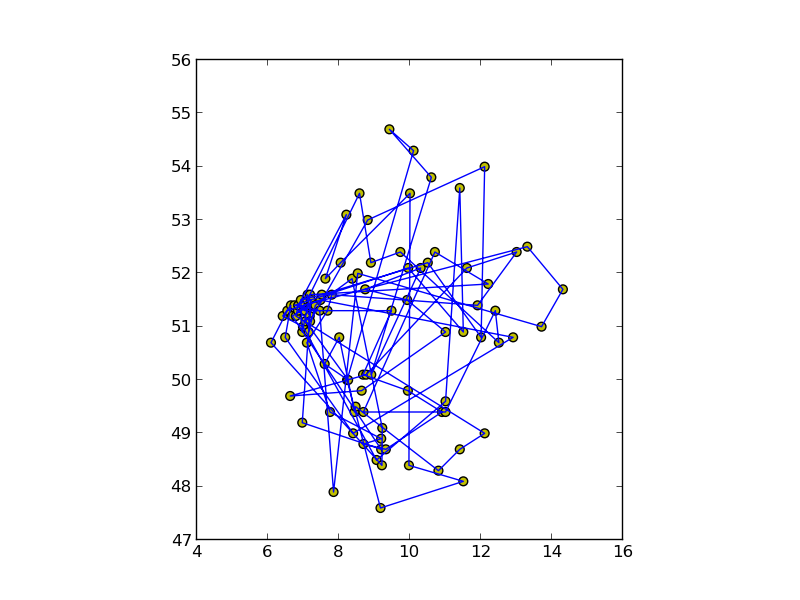
\includegraphics[width=.8\linewidth]{img/ex3/196,29-30-100-200-0,1-0,01.png}
  %\caption{}
  %\label{fig:}
\end{minipage}%
\begin{minipage}{.5\textwidth}
  \centering
  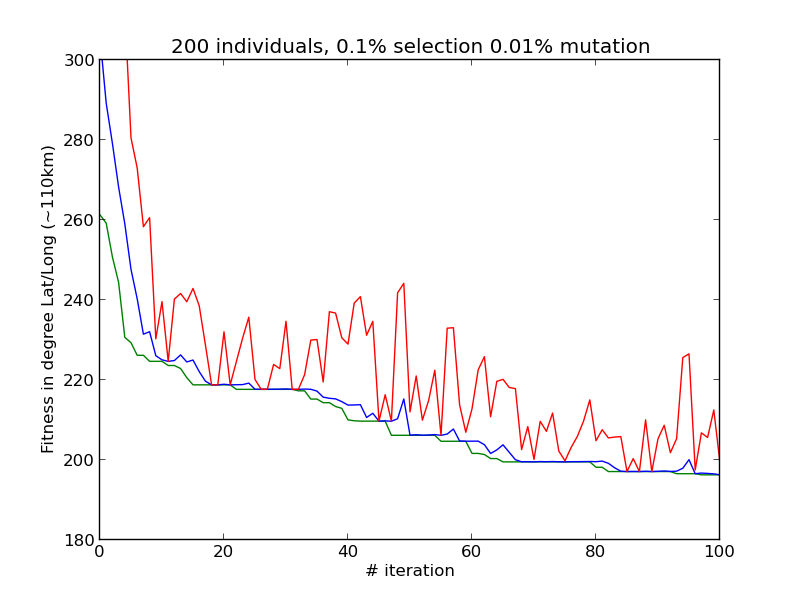
\includegraphics[width=.8\linewidth]{img/ex3/196,29-30-100-200-0,1-0,01-fitness.png}
  %\caption{}
  %\label{fig:} 
\end{minipage}
\caption{A typical run for the complete analysis. 100 iterations with 200 individuals, a selection of 10\% and mutation rate of 1\% (not 0.1 and 0.01 as in the image). The position of the cities are given in Lat/Long, as well as the fitness. The fitness is given as max(red), mean(blue) and min(green).}
\label{fig:typicalfit}
\end{figure}
%Description

\subsubsection{Best result}
From the analysis I concluded to stay with a population size of 200, but focus more on mutation (60\%) then crossover (selection 20\%) with a lot more iteration (1000). After I introduced mutation protection and elitism, I got a mean value close to the min value (small selection) while having mutations with a wide variety (Channel of the red line). The best fitness value of 68.46 $^\circ$ lat/long ($~7530$ km) is quite good to the results discussed in class.

%TSP BEST
\begin{figure}[H]
\centering
\begin{minipage}{.5\textwidth}
  \centering
  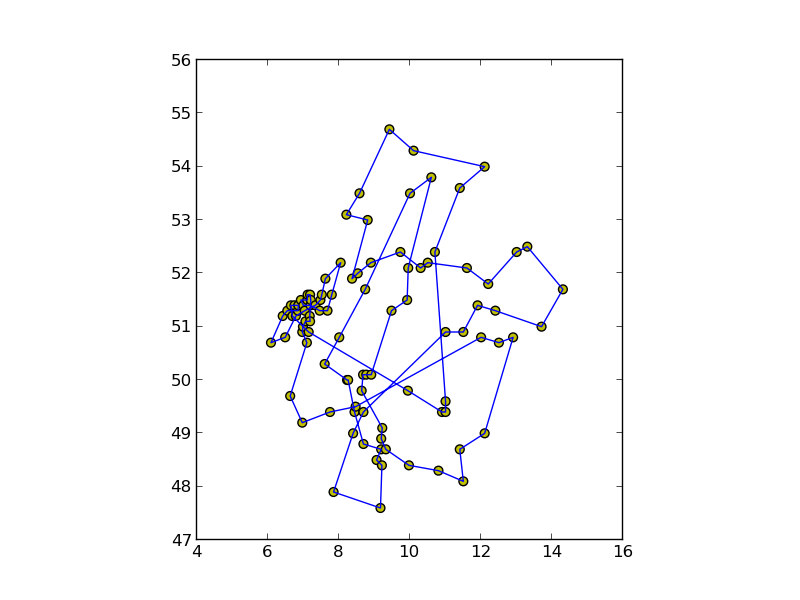
\includegraphics[width=.8\linewidth]{img/ex3/68,46-1-1000-200-0,2-0,6.png}
  %\caption{}
  %\label{fig:}
\end{minipage}%
\begin{minipage}{.5\textwidth}
  \centering
  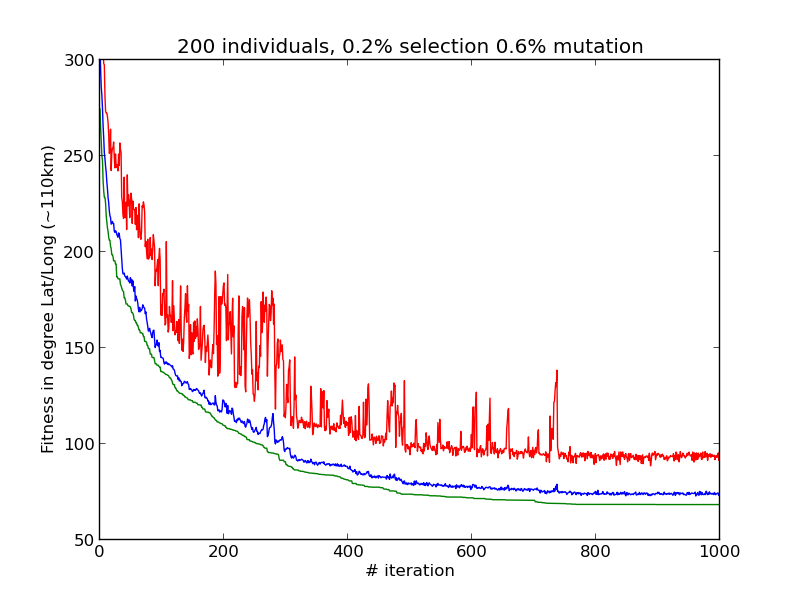
\includegraphics[width=.8\linewidth]{img/ex3/68,46-1-1000-200-0,2-0,6-fitness.png}
  %\caption{}
  %\label{fig:} 
\end{minipage}
\caption{The best run for the travelling salesman. 1k iterations with 200 individuals, a selection of 20\% and mutation rate of 60\% (not 0.2 and 0.6 as in the image). The position of the cities are given in Lat/Long, as well as the fitness. The fitness is given as max(red), mean(blue) and min(green).}
\label{fig:}
\end{figure}
%Description

\subsection{Conclusion}
With the BuildingBlock, Schema Theory, Neutrality this exercise introduced a lot of Theory. In addition with the monitoring of the min, mean and max fitness over time it was possible to significantly improve the performance of an algorithm, even without increasing the complexity of the solution. It was shown that it is not necessary to artificially introduce building blocks by mutating only blocks or using blocks in the crossover.\\
The choice of representations also does not seem to be of importance, as long as one keeps in mind that different representations lay close to different mutations. However it was not possible to compare the computing efficiency of different representations. Also, time fell short to test the effect of introducing multiple solutions with neutral representations.




\section{Evolutionary Algorithm}
%Theoretic description
While the Genetic algorithm focuses on crossover and a big population size, one also can focus on mutations. This is done in Evolutionary algorithms, where a small population is mutated over and over to approach an optimal solution.

\subsection{Problem}
%characteristics of the problem
The problem given is to provide motor commands to a vehicle so that it will pass an undulating path in minimal time. The motor command can be between 0 and 1 an be place at any of the 8191 positions. The fitness function was given, but not to be examined in detail. The track itself (as part of the Fitness function) unknown.

\subsection{Algorithms}
%How do we solve it
Similar to the genetic algorithm, the evolutionary algorithm is iterated over the following steps:

\begin{itemize}
\item evaluation
\item recombination
\item selection
\end{itemize}

There is no crossover and the mutation is no global operation but is moved inside of the selection. The mutation is a critical step in this algorithm and thus gets extra attention. The mutation happens by random drawn from a Gaussian distribution with a mean of the current value and a given sigma. The sigma defines how big the deviation of the mutation can be. Thus a bigger sigma searches for more different solutions while small sigma searches to optimize the current solution with a small variation.\\
The recombination step evaluates the current success rate of the mutations and adapts the sigma to either broaden the search or optimize a local strategy. This happens according to the 1/5th rule:

\begin{itemize}
\item If more than 20\% of the mutations improve, we increase the sigma
\item If less than 20\% of the mutations improve, we decrease the sigma
\end{itemize}

Thus the sigma shall adapt itself to balance the algorithm between optimizing and searching for alternatives.\\


\subsection{Representation}
The genotype was a list of motor commands and positions at which those command would apply. The motor commands by nature where fixed between zero and one, while the position could either be also be between 0 and 1 to make a use of random functions easier or it could also represented as a value between 0 and 8190, in which case one has to take care about scaling but does not risk to not be able to represent some points due to the imprecision of floating values.\\
The representation chosen was a list of positions between 0 and 8190 and the new motor commands from that point on. The list thus has not to be of length 8190, because only points of change in motor commands are relevant.


\subsection{Mutation effects}
The mutations in general turned out to be the key to success with this problem. Whenever the vehicles velocity fell to zero, it would not reach the end and not produce a valid fitness. With that in mind it already becomes clear why randomness is a delicate manner here.\\
For the initialisation for example it is not advisable to choose the positions and velocities at random because all solutions that doe not start at a position of zero and a significant speed are invalid. Thus a default a starting position of 0 and a motor command of 1.0 was chosen. This is unlikely to trap the algorithm in a local minima because the velocity can be mutated later.\\
Mutation can only affect the velocity and the position in the list. This does not allow to increase the list and thus the complexity of the solution. Because it is unlikely that an optimal solution only has one command, a mechanism to introduce more decision points is implemented.\\
At random positions, the previous motor command is duplicated. Thus the mutation at first neutral. Then this new decision point is mutated. To keep the list short, neutral points are again removed every step.

\subsection{Parameters}
%What could be changed
\subsubsection{Iterations}
In all runs, 30 iterations where done.

\subsubsection{Sigma/ Sigma Delta}
We use a starting Sigma for the Gaussian distribution of the random variable and select a Sigma Delta as a factor by which the de- or increase the sigma during recombination.\\
The Sigma values where 0.002, 0.02 and 0.2.\\
The Sigma Delta value where 0.0, 0.01, 0.1, where 0.0 means no adaptation.

\subsubsection{selection Mode}
The selection for Evolutionary algorithms is defined by the schema $\mu separator \lambda$ where $\mu$ is the number of parents (selection) and $\lambda$ is the number of offspring. The separator can either be a plus ($+$ in which case the next selection will be based on parents and offsprings, or a comma ($,$) in which case the selection will be based on the offsprings only.
Of those selection modes the following where tested: '1+1', '1+20', '2+20', '1,20', '2,20'


\subsection{Analysis}
%what happened and why
In this task it quickly turned out that the major difficulty would be to tune the mutations. A majority of all mutations leads to invalid solutions. That leads to a very slow improvement and, if the 1/5th rule is applied to a steady decrease of the sigma value. The evaluation consequently focuses on those two parameters.\\


%SIGMA
\begin{figure}
 \center
 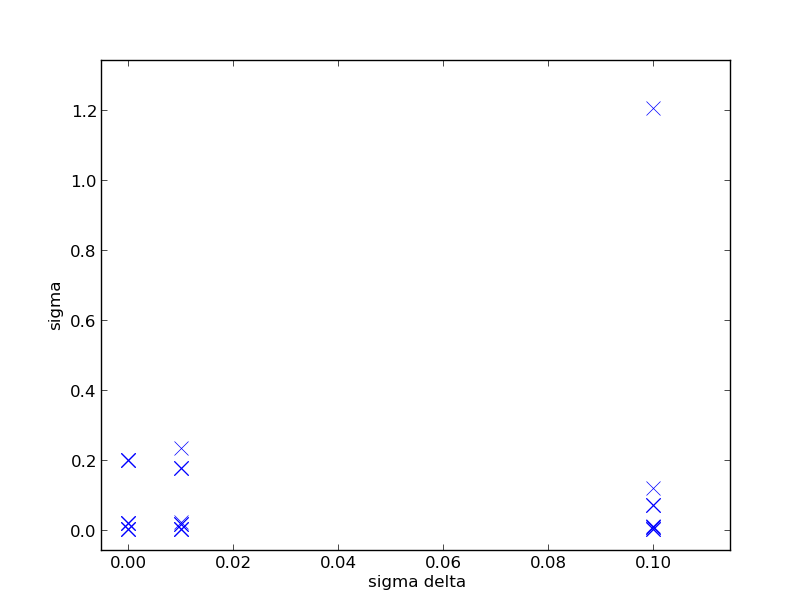
\includegraphics[width=.5\linewidth]{img/ex4/sigmas.png}
 \caption{Final sigma in relation to the sigma delta over all runs.}
\end{figure}



\begin{table}[htbp]
\caption{Fitness over 30 runs each}
\begin{tabular}{r r r|r r }

selection & Sigma $\Delta$ & Sigma & Mean Fitness & Best Fitness \\ \hline
1+1 & 0 & 0.002 & 1228892 & 1228892 \\ 
1+1 & 0.01 & 0.002 & 1228793 & 1228561 \\ 
1+1 & 0.1 & 0.012 & 1225754 & 1221046 \\ 
1+1 & 0 & 0.02 & 1228892 & 1228892 \\ 
1+1 & 0.01 & 0.023 & 1228892 & 1228892 \\ 
1+1 & 0.1 & 0.121 & 1228892 & 1228892 \\ 
1+1 & 0 & 0.2 & 1228892 & 1228892 \\ 
1+1 & 0.01 & 0.234 & 1228892 & 1228892 \\ 
1+1 & 0.1 & 1.206 & 1228892 & 1228892 \\ 
1+20 & 0 & 0.002 & 1224793 & 1220197 \\ 
1+20 & 0.01 & 0.002 & 1220713 & 1213483 \\ 
1+20 & 0.1 & 0.001 & 1225500 & 1222800 \\ 
1+20 & 0 & 0.02 & 1227115 & 1226354 \\ 
1+20 & 0.01 & 0.018 & 1228892 & 1228892 \\ 
1+20 & 0.1 & 0.007 & 1225472 & 1221001 \\ 
1+20 & 0 & 0.2 & \textbf{1188537} & \textbf{1128005} \\ 
1+20 & 0.01 & 0.175 & 1228892 & 1228892 \\ 
1+20 & 0.1 & 0.07 & 1226681 & 1220602 \\ 
2+20 & 0 & 0.002 & 1225606 & 1223490 \\ 
2+20 & 0.01 & 0.002 & 1224471 & 1220651 \\ 
2+20 & 0.1 & 0.001 & 1226304 & 1224964 \\ 
2+20 & 0 & 0.02 & 1228892 & 1228892 \\ 
2+20 & 0.01 & 0.018 & 1227215 & 1221702 \\ 
2+20 & 0.1 & 0.007 & 1211559 & \textbf{1197249} \\ 
2+20 & 0 & 0.2 & 1218575 & \textbf{1190204} \\ 
2+20 & 0.01 & 0.175 & 1228892 & 1228892 \\ 
2+20 & 0.1 & 0.07 & 1228892 & 1228892 \\ 
1,20 & 0 & 0.002 & inf & inf \\ 
\dots & & & \dots & \dots \\
%1,20 & 0.01 & 0.002 & inf & inf \\ 
%1,20 & 0.1 & 0.002 & inf & inf \\ 
%1,20 & 0 & 0.02 & inf & inf \\ 
%1,20 & 0.01 & 0.018 & inf & inf \\ 
%1,20 & 0.1 & 0.007 & inf & inf \\ 
%1,20 & 0 & 0.2 & inf & inf \\ 
%1,20 & 0.01 & 0.175 & inf & inf \\ 
%1,20 & 0.1 & 0.07 & inf & inf \\ 
%2,20 & 0 & 0.002 & inf & inf \\ 
%2,2 & 0.01 & 0.002 & inf & inf \\ 
%2,20 & 0.1 & 0.002 & inf & inf \\ 
%2,20 & 0 & 0.02 & inf & inf \\ 
%2,20 & 0.01 & 0.018 & inf & inf \\ 
%2,20 & 0.1 & 0.007 & inf & inf \\ 
%2,20 & 0 & 0.2 & inf & inf \\ 
%2,20 & 0.01 & 0.175 & inf & inf \\ 
2,20 & 0.1 & 0.07 & inf & inf \\ 
\end{tabular}
\label{}
\end{table}


\subsubsection{Fitness}

\subsubsection{Best result}

%VEHICLE BEST
\begin{figure}
 \center
 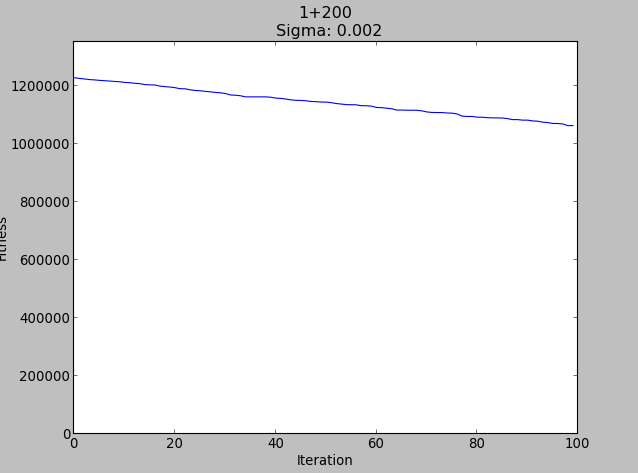
\includegraphics[width=.5\linewidth]{img/ex4/1063459-1+200-0,002.png}
 \caption{Screenshot of the best run with a final fitness of 1063459, and a fixed sigma of 0.002.}
\end{figure}


\subsection{Conclusion}


%CONTENTS
%NOTES


%COPY AND PASTE FROM HERE

%\begin{enumerate}
% \item 
%\end{enumerate}

%\hyperref{link}{text}

%\begin{lstlisting}[language=Python]
%#PYTHON CODE HERE
%\end{lstlisting}

%\lstinputlisting[Language=Python]{ }


%\begin{figure}
% \center
% \includegraphics[width= cm]{ }
% \caption{}
%\end{figure}


%\begin{figure}[H]
%\centering
%\begin{minipage}{.5\textwidth}
%  \centering
%  \includegraphics[width=.8\linewidth]{img/}
%  %\caption{}
%  %\label{fig:}
%\end{minipage}%
%\begin{minipage}{.5\textwidth}
%  \centering
%  \includegraphics[width=.8\linewidth]{img/}
%  %\caption{}
%  %\label{fig:} 
%\end{minipage}
%\caption{}
%\label{fig:}
%\end{figure}
%Description


%BIBLIOGRPAHY?
\bibliographystyle{plain}%amsalpha
\bibliography{Top30.bib}
%\bibentry{}

\end{document}
